%% ----------------------------------------------------------------------------
% BIWI SA/MA thesis template
%
% Created 09/29/2006 by Andreas Ess
% Extended 13/02/2009 by Jan Lesniak - jlesniak@vision.ee.ethz.ch
%% ----------------------------------------------------------------------------
\chapter{Implementation Details}
\label{app:implementation_details}

The software produced for this thesis can be found at [??]. To use the software the following steps should be executed:
\begin{enumerate}
\item The input data should be preprocessed to the correct format, to prevent expensive transformations while the network is learning. For this the scripts in the \textit{prepare/data} directory are useful. They read the images from a central location and scale them down to 227x227 size, including possible conversion to grayscale before storing them on disk.
\item Then the required training and test set can be generated. Scripts are provided in the \textit{prepare/input} directory for different variations of the experiments.
\item In this step the actual different types of experiments are generated, for this purpose an \textit{generate/gen\_experiment.py} script is provided that initializes a directory with a solver.txt and net.txt protobuf files necessary for running Caffe. All the experiments are found in the \textit{experiments} folder, where relevant paths should be updated to reflect the local file system.
\item Eventually the training can be run by invoking \textit{train.py} with the first argument to the solver.txt of the generated experiment. 
\item Finally when training is finished, accuracy can be calculated and some of the visualizations can be produced by running \textit{test.py} with the first argument pointing to the net.prototxt and the second argument to a .caffemodel file produced during training that contain the state of the network.
\end{enumerate}
All the software is made available under the MIT license. Note that the software is considered research in progress and has limited documentation. Small changes might be required to run the software stack on your own computer, however everything to reproduce the results in this work should be present.

\chapter{Additional Visualizations}
\label{app:additional_visualizations}
This appendix provides examples of visualizations not shown earlier in this thesis. Figure \ref{fig:activate_regions} displays important sections of several frames with a similar purpose as the saliency maps shown in Figure \ref{fig:saliency}, but using a different method. Filter activations of the first frame from Figure \ref{fig:frames} are shown for the first and fifth convolutional layer in respectively Figure \ref{fig:conv1_activations} and Figure \ref{fig:conv5_activations}. 

\begin{figure}[b!]
\centering
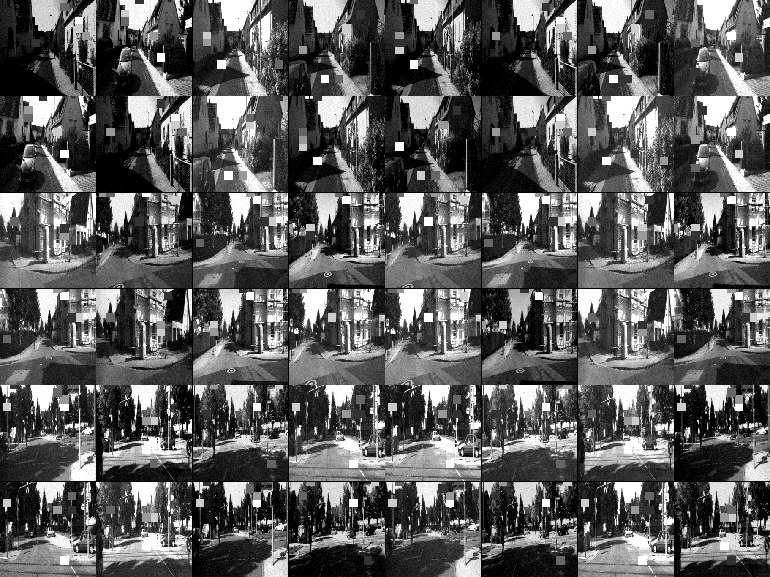
\includegraphics[width=\textwidth]{images/activated_regions.png}
\caption{Several series of frames with blocks from white to black showing the regions with maximum activations of the fifth convolutional filters.}
\label{fig:activate_regions}
\end{figure}

\begin{figure}
\centering
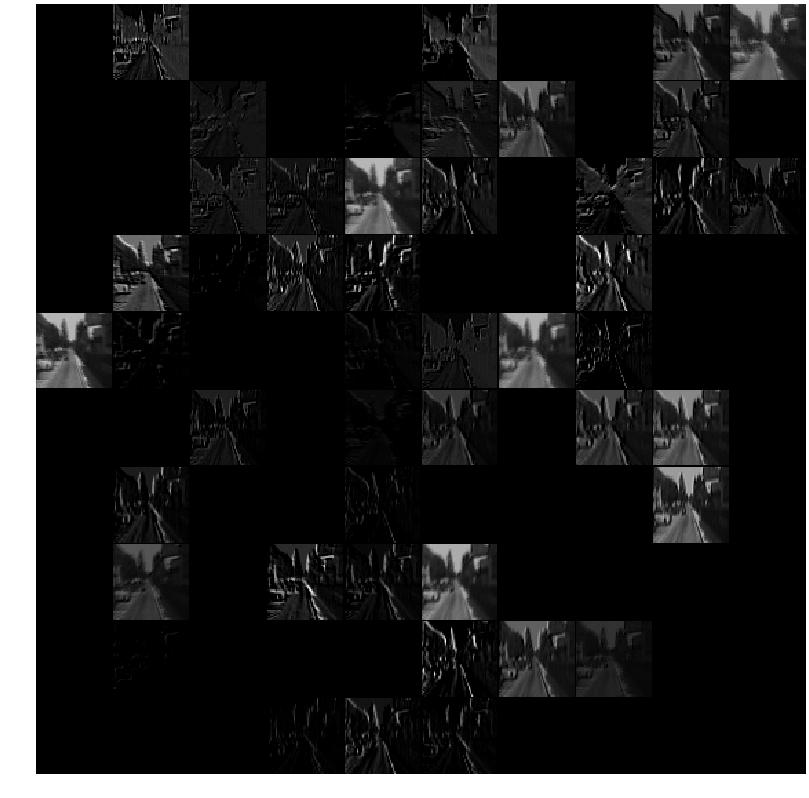
\includegraphics[width=0.75\textwidth]{images/conv1_activations_image1.png}
\caption{Example activations of first layer filters for grayscale feature}
\label{fig:conv1_activations}
\end{figure}

\begin{figure}
\centering
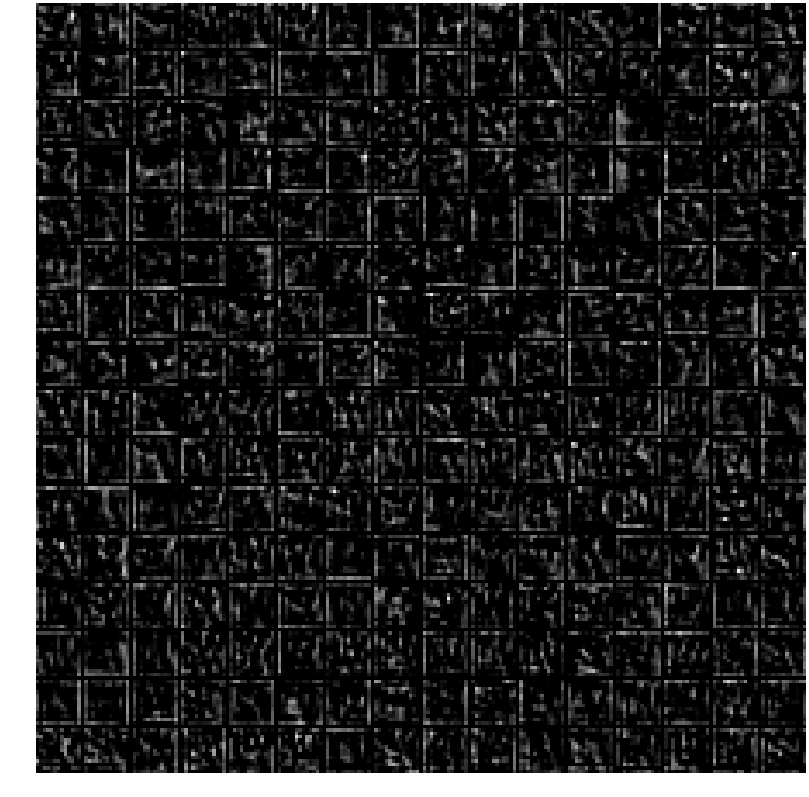
\includegraphics[width=0.75\textwidth]{images/conv5_activations_image1.png}
\caption{Example activations of fifth layer filters for grayscale feature}
\label{fig:conv5_activations}
\end{figure}
